\chapter{Background}

\section{The \Beluga Language}

In \Beluga, theorems are encoded using contextual \LF, its index language, and proofs are encoded as programs.

% TODO:

Let $x$ range over identifiers, $c$ over constants, $X$ over contextual objects, $\psi$ over contexts and $g$ over context schemas.
Figure~\ref{figure:internal-syntax} then provides a brief overview of \Beluga from a theoretical standpoint.

\begin{figure}
\begin{subfigure}{\linewidth}
\begin{tabular}{p{5.5cm} >{\raggedleft}p{1cm} r l}
\LF kinds & $K$ & $\Coloneqq$ & $A \to K \mid \Pi x{:}A. K \mid \mathbf{type}$\\
\LF types & $A, B$ & $\Coloneqq$ & $A\to B \mid \Pi x{:}A. B \mid P$\\
Atomic \LF types & $P$ & $\Coloneqq$ & $a \cdot S$\\
\LF normal terms & $M$ & $\Coloneqq$ & $R \mid \lambda x. M$\\
\LF neutral terms & $R$ & $\Coloneqq$ & $H \cdot S \mid u[\sigma]$\\
\LF heads & $H$ & $\Coloneqq$ & $x \mid c \mid p[\sigma]$\\
\LF spines & $S$ & $\Coloneqq$ & $\cdot \mid M\ S$\\
Substitutions & $\sigma$ & $\Coloneqq$ & $\cdot \mid \mathsf{id}_\psi \mid \sigma, M \mid \mathsf{id}_\psi[\rho]$\\
Substitution closures & $\rho$ & $\Coloneqq$ & $s[\sigma]$\\
Contexts & $\Psi$ & $\Coloneqq$ & $\cdot \mid \psi \mid \Psi, x : A$\\
\end{tabular}
\caption{Internal syntax of contextual \LF in \Beluga.}
\end{subfigure}
\par\bigskip
\begin{subfigure}{\linewidth}
\begin{tabular}{p{5.5cm} >{\raggedleft}p{1cm} r l}
Meta-types & $U$ & $\Coloneqq$ & $g \mid \Psi \vdash A \mid \Psi \vdash \Psi \mid \cdots$\\
Meta-objects & $C$ & $\Coloneqq$ & $\Psi \mid \Psi \vdash M \mid \Psi \vdash \sigma \mid \cdots$
\end{tabular}
\caption{Internal syntax of \Beluga's meta level (excerpt).}
\end{subfigure}
\par\bigskip
\begin{subfigure}{\linewidth}
\begin{tabular}{p{5.5cm} >{\raggedleft}p{1cm} r l}
Computation-level kinds & $\kappa$ & $\Coloneqq$ & $[U] \to \kappa \mid \Pi X{:}U. \kappa \mid \mathbf{ctype}$\\
Computation-level types & $\tau$ & $\Coloneqq$ & $c \mid \tau_1 \to \tau_2 \mid \Pi X{:}U. \tau \mid [U] \mid \tau\ [C] \mid \cdots$\\
Type-checkable expressions & $e$ & $\Coloneqq$ & $i \mid [C] \mid \mathbf{fn}\ x \Rightarrow e \mid \mathbf{mlam}\ X \Rightarrow e$ \\
& & $|$ & $\mathbf{let}\ x = i\ \mathbf{in}\ e \mid \mathbf{case}\ i\ \mathbf{of}\ \overrightarrow{p \Rightarrow e} \mid \cdots$\\
Type-synthesizing expressions & $i$ & $\Coloneqq$ & $x \mid c \mid i \ e \mid e : \tau \mid \cdots$
\end{tabular}
\caption{Internal syntax of \Beluga's computation level (excerpt).}
\end{subfigure}
\caption[Excerpt of \Beluga's internal syntax]{%
Excerpt of \Beluga's internal syntax~\cite{nanevski2008contextual, germain2010implementation, cave2013first, ferreira2013compiling} used in discussions about its theory.
}
\label{figure:internal-syntax}
\end{figure}

\section{The Legacy Implementation of \Beluga} \label{section:beluga-implementation}

This section presents an overview of the implementation of \Beluga before any contribution detailed in this thesis were made\footnote{The implementation of \Beluga at revision hash \href{https://github.com/Beluga-lang/Beluga/tree/3db1ffd08d4c3bde7ad2ceb924bfb95488eef2b2}{3db1ffd08d4c3bde7ad2ceb924bfb95488eef2b2, available on GitHub.}}.
This initial description serves as the basis for all performance and design comparisons made with respect to \Beluga version~\texttt{1.1}.

\Beluga is implemented following the pipeline architectural pattern, whereby processing of a \Beluga signature is implemented in distinct phases, and data flows in a feed-forward fashion throughout.
The compilation of \Beluga programs to machine code is not supported, so the implementation only covers the frontend component of compilation, which is responsible for syntactic and semantic analysis of programs.
Since \Beluga is a dependently-typed language featuring code coverage analysis and termination checking, this semantic analysis process is complex.

\begin{figure}
\centering
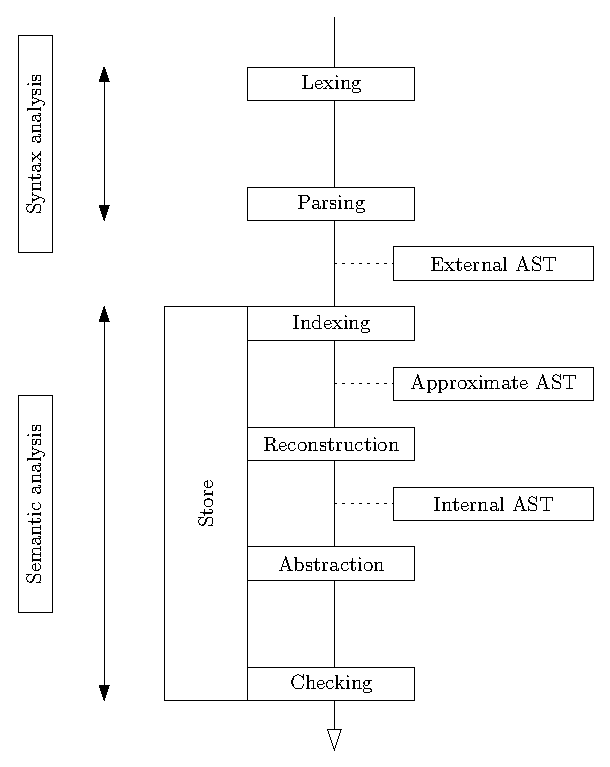
\includegraphics{figures/legacy-beluga-processing-pipeline.eps}
\caption[Overview of the implementation of \Beluga version \texttt{1.0}'s processing pipeline]{%
Overview of the implementation of \Beluga version \texttt{1.0}'s processing pipeline.
The syntax analysis process converts the textual representation of \Beluga programs into an initial \acs{AST}.
The semantic analysis process refines this \acs{AST} by performing type-directed signature reconstruction, using global mutable data structures that include a store of signature entries.
}
\label{figure:legacy-beluga-processing-pipeline}
\end{figure}

As illustrated in figure~\ref{figure:legacy-beluga-processing-pipeline}, the processing of a \Beluga signature starts with syntax analysis, which is comprised of a tokenization and parsing phase that converts the textual representation of the signature to an \ac{AST}, called the external \ac{AST}.
The model for this \ac{AST} contains ambiguous nodes, meaning that some \ac{AST} node variants capture multiple parse trees.
Specifically, the application of \LF type-level and term-level constants is represented as a list of parsemes.
Parsing of signature-level declarations also features mixing/unmixing flags (auxiliary data types for bookkeeping) to postpone some elements of disambiguation to phases after context-free parsing.

Indexing in \Beluga is the process where the concrete syntax is elaborated to an approximate syntax in which most variables are replaced with de Bruijn indices.
Some de Bruin indices computations are postponed until the abstraction phase.
Indexing is run after parsing, and is additionally responsible for disambiguating the juxtaposition of \LF parsemes at the precedence level of applications (which may contain user-defined operators), as well as disambiguating \LF types from terms and resolving constants.
This design is sensible since computing de Bruijn indices requires a stateful traversal of the \ac{AST} that accumulates lists of bindings to produce the referencing environment.
Using the centralized store of declarations, some measure of identifier overloading is supported using a pre-defined order of lookups in the referencing environment based on the kind of identifier that is expected for a given \ac{AST} node.
For instance, computation-level identifiers are resolved by looking up in order the store of computation-level variables, the store of program constants, and then the store of data type constructors.
Since names appearing in the \LF level are not part of this name resolution strategy, then an identifier can be overloaded to stand for an \LF term as well as a computation-level expression.

After indexing, the reconstruction~\cite{pientka2013insider} phase is run to reconstruct holes in types and terms, both at the \LF level and the computation level.
These holes stand for arguments omitted by the user, and provide an elegant way of abbreviating otherwise tedious aspects of programming with dependent types.
At the \LF level, approximate types are constructed to partially check the kinding of \LF types and the typing of \LF terms, as well as for guiding the synthesis of normal terms that check against a given type using typing constraints.
Type-driven unmixing of overloaded syntactic forms occurs at the meta-level, whereby meta-objects are disambiguated from substitutions during reconstruction.
The approximate \ac{AST} provides a disambiguated representation of the overall \Beluga signatures, which helps in keeping track of the various changes made during this complicated phase.

A nearly complete internal \ac{AST} is produced at the end of reconstruction.
An abstraction phase~\cite{germain2010implementation} is run to abstract over free variables, which effectively introduces binders for implicit parameters.
This phase completes the desugaring of \Beluga programs since it finishes the computation of de Bruijn indices for variables across all levels.
The main technical challenge abstraction runs into is determining the order in which introduced binders must appear so that dependencies on terms are preserved in inferred dependent types.
This includes identifying and handling circular dependencies in abstracted parameters.

Finally, a semantic checking phase is run to ensure signature reconstruction and abstraction yielded valid programs.
This includes performing type-checking, coverage-checking and totality-checking.
These processes guarantee, respectively, that \LF-level and computation-level expressions are well-typed, that case analyses are exhaustive, and that functions annotated with a totality declaration terminate for all inputs.
Typing and coverage constraints generated during theses checking processes are statefully shared throughout this phase.
Leftover and unresolved constraints that are still in the state after having fully processed a program unit are used to signal to the user that that program is unsound within \Beluga's system.

The flow of data in the implementation of \Beluga is complex, like in most software systems.
Starting with the indexing phase, data is shared between the phases of signature reconstruction using a global mutable store.
This auxiliary data structure is a set of tables mapping constant identifiers to meta-data like in a relational database.
Crucially, the referencing environment used during indexing is computed using this store.
At any given point during the processing pipeline, the state of the store is valid since program units are processed sequentially.
New program units may be safely appended afterwards in interactive sessions.

The \Beluga system provides two ways to interactively perform queries on an existing \Beluga signature, or to augment it with new theorems.
These are the legacy \ac{REPL} and the \Harpoon system~\cite{errington2021harpoon}, the latter of which was designed as a replacement for the former.
Both systems allow the user to input \LF-level terms or computation-level expressions and get their type inferred with respect to an already elaborated \Beluga signature.
\Harpoon further enables the interactive definition and proving of theorems using sets of tactics aimed at automating proof development.
Both the \ac{REPL} and \Harpoon depend on the earlier processing phases of \Beluga and the flow of information therein.

This thesis focuses on the first few phases of the \Beluga processing pipeline, specifically parsing and indexing, and how re-architected solutions to those phases provide better support for some of \Beluga's and \Harpoon's existing features.

\section{State Management and Incremental Program Development}

Users benefit from interacting with the code they are editing by way of auxiliary software that performs actions on it.
Incremental program development in programming language tooling is the problem of applying edit actions to programs while only re-processing a minimal portion of the program under edit.
The kinds of edit actions that can be implemented vary from one programming language to the other depending on the language's features.
Typically, edit actions include software refactoring commands such as variable renaming, reordering functions in a file, selecting a list of statements from one function and extracting them to a separate function, pretty-printing and formatting the textual representation of code, etc.
Sound and efficient handling of these edit actions is instrumental to the productivity of users working on large scale software systems.
This problem of incremental program development arises in \Beluga and \Harpoon because of the interactive tooling they provide for editing proofs, which are represented as programs.
%In compiler design, the problem analogous to incremental program development is incremental compilation.

% What is the key problem in incremental program development?
Throughout syntactic and semantic analyses pipelines, data is accumulated during the processing of any given program unit.
%This data typically includes lookup tables for resolving identifiers to their declaration site, auxiliary data structures to speed up algorithms, sets of constraints on types used during type-checking and type inference, etc.
This data raises one of the main challenges in implementing incremental program development in that a program unit may only be revisited with the processing state it was defined in.
This means, for instance, that a procedure performing name lookups or mutations on an \ac{AST} at a given node may only do so using the variables and declarations in scope at that \ac{AST} node, just as the user does when editing the textual representation of that \ac{AST} node.
As such, edit actions on an \ac{AST} must preserve its semantic correctness properties so that serializing and subsequently deserializing it produces the same \ac{AST} and processing state.
%This problem arises when a compiler is extended to support user interactions or non-sequential compilation steps.

% What are some non-sequential compilation steps that need to be scope safe?
%Non-sequential processes in compiler design refer to compilation steps that occur concurrently, or occur using a subset of the data from previous compilation phases.
%In general programming languages, these processes typically appear in the incremental compilation of programs whose dependency relation on compilation units may be arranged in a lattice.
%To implement this, a \ac{DAG} of the compilation units is constructed where edges denote dependency.
%A topological ordering is then computed for that \ac{DAG}, and used to create a compilation schedule, which may feature forked compilation processes for independent compilation units.
%This enables parallelism to be used to reduce compilation time, and potentially the number of compilation units that need to be recompiled after an edit action is performed.
%Implementing these features may require caching of compilation results and restoring processing states from those caches, which naturally raises the concern of cache invalidation.
%Indeed, an incremental compilation process needs to be resumed in the state it originally happened, and changes that occur as a result of this compilation need to be propagated to the rest of the compiler's state.
%This in turn triggers additional compilation steps for units that have explicit or transitive dependencies on the newly compiled unit.

% What is the general solution to the name resolution problem in incremental program development?
A preliminary step to supporting incremental program development is to parameterize the processing routines with respect to a visitor state.
As such, those routines can be used in an out-of-order fashion as opposed to when the program is processed during compilation tasks.
This is because the routine can be visited with a different state than the one that is naturally constructed when sequentially processing program units.
For instance, a routine like conflict-avoiding variable renaming can be dependent on a referencing environment to perform variable and constant lookups.
If such a routine is invoked during an interactive program development session, then a separate routine can be implemented to rebuild the referencing environment without having to re-process the entire program and its dependencies.
In this case, the edit action requires visiting a selected \ac{AST} node with the referencing environment as visitor state.
The issue then becomes how to efficiently construct and preserve the correctness of such visitor states.
As it pertains to \Beluga and \Harpoon, this specifically affects \ac{REPL} sessions instantiated at program holes.

% An open stateful function is a function parameterized over some state, and the lifecycle of the mutable state is extrinsinc.
% A closed stateful function is a function that internally uses mutable states, whose lifecycle is intrinsically maintained.
